\documentclass[10pt]{article}\usepackage[margin=.55in]{geometry}\usepackage[T1]{fontenc}\usepackage{graphicx}\setlength{\parindent}{0pt}\setlength{\parskip}{4pt}\sloppy\begin{document}{\large Runtime assembler v2 final completion guard}\par The assembler now checks monotonic/absolute expiry and pending signals after synchronous input verification returns, after the final workflow readback, and before accepting built\_pending\_qualification. Eighteen mocked tests pass: the original fourteen plus final-check monotonic expiry, final-check signal, absolute expiry with monotonic time remaining, and valid completion. Exact source/test/output hashes and invocation are in test-receipt.json.\par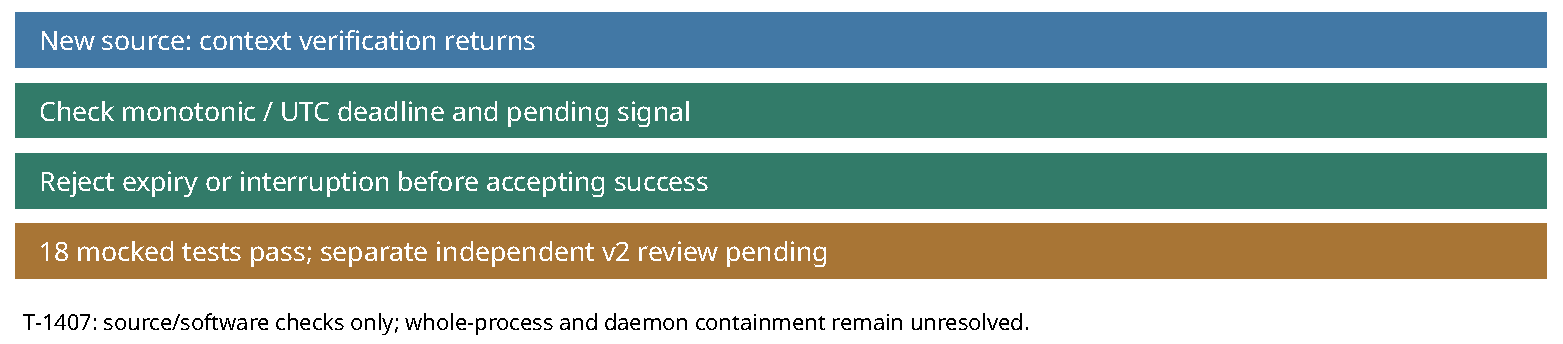
\includegraphics[width=.9\linewidth]{diagram.pdf}\par This is a new implementation packet. The original runtime-replacement-assembler packet is unchanged. Its independent review is archived separately in runtime-assembler-independent-review; that reviewer authored this fix and therefore does not independently approve v2. New independent source review is required. The copied binding remains admitted=false with null review fields, and its assembler hash is refreshed.

Internal checks bound client dispatch and reject observed late/interrupted completion. They do not forcibly interrupt synchronous filesystem reads, the input checker, or receipt writes. External whole-process containment and Docker daemon containment/reconciliation remain unresolved prospective admission obligations, together with finite resource/cost accounting, trusted reviewer provenance and prior-owner reconciliation. An image remains pending qualification after success. No Docker, sudo, build, qualifier, cloud or scientific workload ran; no execution allowance was renewed or approved.
\end{document}